%% BioMed_Central_Tex_Template_v1.06
%%                                      %
%  bmc_article.tex            ver: 1.06 %
%                                       %

%%IMPORTANT: do not delete the first line of this template
%%It must be present to enable the BMC Submission system to
%%recognise this template!!

%%%%%%%%%%%%%%%%%%%%%%%%%%%%%%%%%%%%%%%%%
%%                                     %%
%%  LaTeX template for BioMed Central  %%
%%     journal article submissions     %%
%%                                     %%
%%          <8 June 2012>              %%
%%                                     %%
%%                                     %%
%%%%%%%%%%%%%%%%%%%%%%%%%%%%%%%%%%%%%%%%%


%%%%%%%%%%%%%%%%%%%%%%%%%%%%%%%%%%%%%%%%%%%%%%%%%%%%%%%%%%%%%%%%%%%%%
%%                                                                 %%
%% For instructions on how to fill out this Tex template           %%
%% document please refer to Readme.html and the instructions for   %%
%% authors page on the biomed central website                      %%
%% http://www.biomedcentral.com/info/authors/                      %%
%%                                                                 %%
%% Please do not use \input{...} to include other tex files.       %%
%% Submit your LaTeX manuscript as one .tex document.              %%
%%                                                                 %%
%% All additional figures and files should be attached             %%
%% separately and not embedded in the \TeX\ document itself.       %%
%%                                                                 %%
%% BioMed Central currently use the MikTex distribution of         %%
%% TeX for Windows) of TeX and LaTeX.  This is available from      %%
%% http://www.miktex.org                                           %%
%%                                                                 %%
%%%%%%%%%%%%%%%%%%%%%%%%%%%%%%%%%%%%%%%%%%%%%%%%%%%%%%%%%%%%%%%%%%%%%

%%% additional documentclass options:
%  [doublespacing]
%  [linenumbers]   - put the line numbers on margins

%%% loading packages, author definitions

%\documentclass[twocolumn]{bmcart}% uncomment this for twocolumn layout and comment line below
\documentclass{bmcart}

%%% Load packages
%\usepackage{amsthm,amsmath}
%\RequirePackage{natbib}
%\RequirePackage[authoryear]{natbib}% uncomment this for author-year bibliography
%\RequirePackage{hyperref}
\usepackage[utf8]{inputenc} %unicode support
\usepackage{graphicx}
%\usepackage[applemac]{inputenc} %applemac support if unicode package fails
%\usepackage[latin1]{inputenc} %UNIX support if unicode package fails


%%%%%%%%%%%%%%%%%%%%%%%%%%%%%%%%%%%%%%%%%%%%%%%%%
%%                                             %%
%%  If you wish to display your graphics for   %%
%%  your own use using includegraphic or       %%
%%  includegraphics, then comment out the      %%
%%  following two lines of code.               %%
%%  NB: These line *must* be included when     %%
%%  submitting to BMC.                         %%
%%  All figure files must be submitted as      %%
%%  separate graphics through the BMC          %%
%%  submission process, not included in the    %%
%%  submitted article.                         %%
%%                                             %%
%%%%%%%%%%%%%%%%%%%%%%%%%%%%%%%%%%%%%%%%%%%%%%%%%


%\def\includegraphic{}
%\def\includegraphics{}



%%% Put your definitions there:
\startlocaldefs
\endlocaldefs


%%% Begin ...
\begin{document}

%%% Start of article front matter
\begin{frontmatter}

\begin{fmbox}
\dochead{Research}

%%%%%%%%%%%%%%%%%%%%%%%%%%%%%%%%%%%%%%%%%%%%%%
%%                                          %%
%% Enter the title of your article here     %%
%%                                          %%
%%%%%%%%%%%%%%%%%%%%%%%%%%%%%%%%%%%%%%%%%%%%%%

\title{Avoidable deaths caused stagnation and reversal on survival improvements among adults in Mexican states, 1990-2015}

%%%%%%%%%%%%%%%%%%%%%%%%%%%%%%%%%%%%%%%%%%%%%%
%%                                          %%
%% Enter the authors here                   %%
%%                                          %%
%% Specify information, if available,       %%
%% in the form:                             %%
%%   <key>={<id1>,<id2>}                    %%
%%   <key>=                                 %%
%% Comment or delete the keys which are     %%
%% not used. Repeat \author command as much %%
%% as required.                             %%
%%                                          %%
%%%%%%%%%%%%%%%%%%%%%%%%%%%%%%%%%%%%%%%%%%%%%%

\author[
   addressref={aff1},                   % id's of addresses, e.g. {aff1,aff2}
   corref={aff1},                       % id of corresponding address, if any
   noteref={n1},                        % id's of article notes, if any
   email={jmaburto@health.sdu.dk}   % email address
]{\inits{JMA}\fnm{Jos\'e Manuel} \snm{Aburto}}
\author[
   addressref={aff2},
   email={riffe@demogr.mpg.de}
]{\inits{TR}\fnm{Tim} \snm{Riffe}}

%%%%%%%%%%%%%%%%%%%%%%%%%%%%%%%%%%%%%%%%%%%%%%
%%                                          %%
%% Enter the authors' addresses here        %%
%%                                          %%
%% Repeat \address commands as much as      %%
%% required.                                %%
%%                                          %%
%%%%%%%%%%%%%%%%%%%%%%%%%%%%%%%%%%%%%%%%%%%%%%

\address[id=aff1]{%                           % unique id
  \orgname{Department of Public Health \& Max Planck Odense Center on the Biodemography of Aging at University of Southern Denmark}, % university, etc
  \street{J.B. Winsl{\o}ws Vej 9},                     %
  \postcode{5000}                                % post or zip code
  \city{Odense},                              % city
  \cny{Denmark}                                    % country
}
\address[id=aff2]{%
  \orgname{Max Planck Institute for Demographic Research},
  \street{ Konrad-Zuse-Stra{\ss}e 1},
  \postcode{18057}
  \city{Rostock},
  \cny{Germany}
}

%%%%%%%%%%%%%%%%%%%%%%%%%%%%%%%%%%%%%%%%%%%%%%
%%                                          %%
%% Enter short notes here                   %%
%%                                          %%
%% Short notes will be after addresses      %%
%% on first page.                           %%
%%                                          %%
%%%%%%%%%%%%%%%%%%%%%%%%%%%%%%%%%%%%%%%%%%%%%%

\begin{artnotes}
%\note{Sample of title note}     % note to the article
\note[id=n1]{Equal contributor} % note, connected to author
\note[id=n2]{Equal contributor} 
\end{artnotes}

\end{fmbox}% comment this for two column layout

%%%%%%%%%%%%%%%%%%%%%%%%%%%%%%%%%%%%%%%%%%%%%%
%%                                          %%
%% The Abstract begins here                 %%
%%                                          %%
%% Please refer to the Instructions for     %%
%% authors on http://www.biomedcentral.com  %%
%% and include the section headings         %%
%% accordingly for your article type.       %%
%%                                          %%
%%%%%%%%%%%%%%%%%%%%%%%%%%%%%%%%%%%%%%%%%%%%%%

\begin{abstractbox}

\begin{abstract} % abstract
%\parttitle{First part title} %if any
We analyze trends in mortality for three large age groups from 1990 to 2015 for all 32 Mexican states, and compare these with a low mortality benchmark. We assess the impact of avoidable mortality- conditions amenable to medical service, those sensitive to public health policies and changes in behaviors- on survival at the state level by sex. We apply demographic measures and use standard decomposition techniques to disentangle age-cause-specific effects on survival. We find improvements for the population aged 0 to 14, as they continuously approached full survival. However, the adult population aged 15 to 39 shows deterioration among males after 2006 in almost every state as a result of an increase in homicide mortality. Females on the whole converged toward the low mortality benchmark in the same age group, albeit with some exceptions. Adults aged 40 to 74 show an unexpected decrease in the low mortality benchmark, indicating universal deterioration caused by ischemic heart diseases, diabetes, cirrhosis and homicide mortality. We find large health disparities between states, particularly in the adult population.

%\parttitle{Second part title} %if any
%Text for this section.
\end{abstract}

%%%%%%%%%%%%%%%%%%%%%%%%%%%%%%%%%%%%%%%%%%%%%%
%%                                          %%
%% The keywords begin here                  %%
%%                                          %%
%% Put each keyword in separate \kwd{}.     %%
%%                                          %%
%%%%%%%%%%%%%%%%%%%%%%%%%%%%%%%%%%%%%%%%%%%%%%

%to think about
\begin{keyword}
\kwd{Avoidable mortality}
\kwd{Adult health}
\kwd{Life expectancy}
\end{keyword}

% MSC classifications codes, if any
%\begin{keyword}[class=AMS]
%\kwd[Primary ]{}
%\kwd{}
%\kwd[; secondary ]{}
%\end{keyword}

\end{abstractbox}
%
%\end{fmbox}% uncomment this for twcolumn layout

\end{frontmatter}

%%%%%%%%%%%%%%%%%%%%%%%%%%%%%%%%%%%%%%%%%%%%%%
%%                                          %%
%% The Main Body begins here                %%
%%                                          %%
%% Please refer to the instructions for     %%
%% authors on:                              %%
%% http://www.biomedcentral.com/info/authors%%
%% and include the section headings         %%
%% accordingly for your article type.       %%
%%                                          %%
%% See the Results and Discussion section   %%
%% for details on how to create sub-sections%%
%%                                          %%
%% use \cite{...} to cite references        %%
%%  \cite{koon} and                         %%
%%  \cite{oreg,khar,zvai,xjon,schn,pond}    %%
%%  \nocite{smith,marg,hunn,advi,koha,mouse}%%
%%                                          %%
%%%%%%%%%%%%%%%%%%%%%%%%%%%%%%%%%%%%%%%%%%%%%%

%%%%%%%%%%%%%%%%%%%%%%%%% start of article main body
% <put your article body there>

%%%%%%%%%%%%%%%%
%% Background %%

\section*{Background}
The 20th century was marked by sizable improvements in mortality, living
conditions and health in most Latin American countries \cite{who2000}. 
In Mexico, these improvements have slowed down recently as a result of opposing
trends in particular causes of death. For instance, homicide and diabetes
increased during the first decade of the 2000's, even as infectious and
respiratory diseases continued to fall over the same period. While life
expectancy at birth increased by 4.3 years for males (from 67.6 to 71.9) and 3.4
for females (from 73.8 to 77.2) between 1990 and 2000 \cite{SOMEDE},
between 2000 and 2010, life expectancy at birth entered into a period of
stagnation for males and slowed progress for females \cite{canudas2014}. 


This
period coincides with the implementation of different public health
interventions, such as the Universal Vaccination Program and Seguro
Popular, which aim to provide primary and secondary
health care to the uninsured population and allocate funds to cover catastrophic
health expenditures \cite{knaul2005}. Further, conditional cash transfer programs were introduced to supply incentives for families to reinvest in education, health, and nutrition in 1997 \cite{neufeld2012}. Some evidence
suggests that Mexico experienced substantial decreases in infant and child
mortality, along with improvements that contributed to the reduction of
mortality and in the prevalence of acute malnutrition between 1980 and 2000
because of these interventions \cite{sepulveda2006}. Similarly, by 2012 Seguro Popular had provided health insurance coverage to an additional 52 million
people in Mexico that previously did not have any access to public health care and, as a result, there has been a reduction in catastrophic health expenditures \cite{knaul2012}.

These actions underscore broad progress in public health interventions, but they mask heterogeneity between Mexican states and the epidemiological patterns for different age groups. Therefore, it is necessary to assess the varied impacts that these interventions may have had on mortality in Mexican states \cite{urquieta2015evolution}. For instance, conditional cash transfers are focused on the poorest states, and Seguro Popular was introduced at different times in different states. In addition, Mexico faces a rapid aging process in which we can anticipate the interaction between infectious diseases and noncommunicable conditions \cite{Bygbjerg1499} on the adult population.\footnote{The percentage of the population aged 60 or older will go from 10\% in 2015 to 15\% in 2030 according to projections made by \cite{CONAPO}} Identifying specific opportunities to improve and put forward solutions to reduce the gap of  the unequal impact of public health interventions on health is a necessary step to promote equitable increases in survival among the Mexican population.% the high degree of social and health inequalities present in the country \cite{Frenk2006} 
% In addition,  given the improvements in health care coverage, the strong role %of institutions, and ongoing public
 %health interventions, 
 
 One approach to assess the impact of health care and other interventions is by operationalizing the
 concept of Avoidable or Amenable Mortality (hereafter abbreviated AM)
 \cite{nolte&mckee2004, nolte&mckee2008,elo2014}. This categorization of mortality aims to measure the quality of health service systems by selecting certain
 causes of death that should not occur in the presence of effective and
 timely health care. Among industrialized countries, such as United States,
 Australia, France, Japan, a reduction in AM rates was
 observed over the past 20 years
 \cite{nolte&mckee2008}. Avoidable mortality rates fell, on average, by 17\%
 for males and 14\% for females in these countries. Despite mortality reductions from cancers and circulatory diseases for
 both sexes, heterogeneity between countries persists, with the United
 States showing the smallest reductions (around 5\%) for both sexes  \cite{nolte&mckee2008}. 
 
 In Mexico, the components of avoidable mortality had different trends since the
late 1990's. Between 2000 and 2004 AM decreased, particularly from
infectious diseases and nutrition-related conditions \cite{francomarina2006}, while it increased between 1998 and 2010 due to diabetes, circulatory diseases, perinatal and respiratory conditions
\cite{agudelo2014efecto}. Increases in the latter causes
of death were particularly concentrated in the poorest states of the country
\cite{davila2014mortalidad}. We aim to extend these studies
by a more focused segmentation of AM into health intervention-related AM and
behavior-related AM. Also, we extend analysis to all 32 states, by sex, and over
the full 26-year period from 1990 to 2015. Finally, we compare state mortality patterns
with an easy-to-understand low-mortality benchmark calculated for large age groups (e.g., 0-14, 15-39, 40-75). This low mortality
benchmark is calculated on the basis of the lowest observed mortality within
ages and causes, selected from the full set of 32 Mexican states. This concept has been previously used in mortality studies \cite{whelpton1947}, and further developed elsewhere 
\cite{wunsch1975minimum,vallin2008minimum}. Deviations from the low-mortality benchmark indicate a strong potential for improvement. We apply demographic measures and
standard decomposition techniques to isolate the cause and age-specific deviations between states and the low mortality optimal lifetable for each year.

We hypothesize age-dependent variations in mortality outcomes.
In particular, we expect convergence between states and improvement in survival
for young people, since public health interventions are mainly focused in infant
mortality and child health. For instance, the vaccination program and the health
reform aim to fully cover children in the entire country, and recent
evidence suggests a decrease in mortality between ages 0 to 14 due to a decline
in infectious and respiratory diseases \cite{gonzalez2016mexico}. On the contrary, we
expect little improvements in survival for the  young-adult population due to the unprecedented rise in homicide mortality, and on the older adults because of the increase in diabetes mortality along with endocrine/metabolic diseases in these ages in the country \cite{gonzalez2011health,gonzalez2016mexico}. Although every
state has the commitment to providing universal coverage and equitable access to
health care since the early 2000's, we anticipate disparities between states
in mortality improvements due to state differences in epidemiological patterns  \cite{gomez2016dissonant} and differences in how  health care programs have been delivered to the population
\cite{Frenk2006}.


\section*{Data \& Methods} 
Our analyses are based on publicly available anonymized datasets. We used deaths microdata available from official files produced by the
Mexican Statistical Office from 1990 to 2015 \cite{INEGI}. These data contain
information on causes of death by single age, sex, and state of residence at the
time of death. Population estimates from 1990 to 2015 came from the Mexican Statistical Office as well \cite{INEGI}. These estimates adjust for age misstatement, undercounting, and interstate and international migration. Death counts and estimated of the population exposed to risk were used to calculate cause-age-specific death rates by sex and state from 1990 to 2015.

\subsection*{Classification of Causes of Death}

To separate causes of death that are susceptible to medical intervention (such as
infectious and respiratory diseases) and those related to health behaviors and
intersectoral policies (such as homicides, lung cancer) we use the concept of
``Avoidable/Amenable Mortality'' (AM) \cite{nolte&mckee2004, nolte&mckee2008}. We group causes of death into ten categories based on a previous classification  \cite{elo2014}, that has recently been complemented to Mexico's case \cite{Aburto2015}, as listed in Table~\ref{tab:causes}, with relative frequencies by sex for the period 2000-2015.



We separate diabetes, ischemic heart diseases (IHD), HIV/AIDS, lung
cancer, and cirrhosis because these causes are susceptible to both health behavior
and medical service, and because the first two represent major causes of death
in Mexican adults \cite{gomez2016dissonant}. We also separate
homicide, road traffic accidents, and suicide because they have emerged as
leading causes of death among young people, and the first two had a sizeable
impact on life expectancy recently in Mexico \cite{Aburto2015}. All causes of death were classified using the International Classification of Diseases, revision 9 for the period 1990-1997 and the tenth revision for 1998-2010 (see SI Table 1 for details on ICD codes for each cause). To avoid spurious results concerning the change in coding practices between the ninth and tenth revision, we performed a sensitivity analysis and did not find major changes in mortality trends by AM classification (See SI figure 1). Although ill-defined causes represent a small percent of the total deaths (2\% in 1992 \cite{rivera2002epidemiological}), we decided to leave them in the residual category because if we spread them proportionally among the other causes of death could over estimate our results.

We truncated analysis at age 75 because classification of causes of deaths and age reporting are considered to be inaccurate in death registration at older ages \cite{tobias2001} and most changes in life expectancy are likely due to changes in mortality patterns below the age of 75 \cite{Aburto2015}. This does not mean that the population above age 75 should not be included in public health priorities.

\subsection*{Age Groups}

We break life expectancy into three large age groups to capture mortality differences along the lifespan based on previous research. The first group refers to people aged 0-14. This group is likely to represent improvements in causes amenable to medical service (e.g. infectious diseases and conditions of perinatal period) \cite{canudas2014}. The second group, aged 15-39, is used to capture the effect of homicide mortality and external causes, historically related to the young-hump in the force of mortality, which have had an important impact on state-life expectancy in the first decade of the 2000s \cite{Aburto2015}. Finally, the third group is for older adults aged 40-74. We focus on older adults because are likely to represent a vulnerable group since mortality rates at adult ages deteriorated in recent years from non-communicable diseases and injury-related mortality \cite{gonzalez2011health,gomez2016dissonant}.


\subsection*{Demographic Methods}
We smooth cause-specific death rates over age and time for each
state and sex separately using the 2-d p-spline
to avoid random variations between ages \cite{GC2012}. Smoothed death rates are
then constrained to sum to the unsmoothed all-cause death rates. We then calculate period life tables up to
age 74 for males and females from 1990 to 2015 following standard demographic methods \cite{preston2001}. We calculate the average years lived in each age group (temporary life expectancy) \cite{arriaga1984} (See SI for a technical overview) and estimate cause-specific contributions to the difference between
state-specific temporary life expectancy and  the low mortality benchmark using
 standard decomposition techniques \cite{horiuchi2008}. Finally, to measure the level of disparities between states over time, we estimate the coefficient of variation and the Gini coefficient on average survival for each age-group in each year. 

\subsection*{Low mortality benchmark}
Our low-mortality benchmark is calculated in the basis of the lowest observed mortality rates by age, cause of death, from among all states for a given sex and year.


%The low mortality rates $\mu(x)^\star$, are calculated as the sum of $C$ cause-specific minimum %mortality rates at age $x$, under the assumption that causes of deatg are independent of one another:
%\begin{equation}
%\label{eq:mxmin}
%\mu(x)^{\star} = \sum_c=1^C min(\mu(x,c,s))
%\end{equation}
%where $x$ is age, $c$ is the given cause of death, and $s$ indexes the set of 32 states from which %the minimum is selected. 

The resulting minimum mortality rate schedule has a unique age profile, and it determines our benchmark temporary life expectancy. The minimum mortality schedule can be treated as the best presently achievable mortality assuming perfect diffusion of the best available practices and technologies within a given set of populations \cite{vallin2008minimum}. It is an imaginary quantity because no particular population is expected to achieve this mortality pattern. However, this value is a practical reference because it is based neither on a projection of improvements into the future nor on an arbitrary and likely dissimilar population. We refer to the state with the highest life expectancy in a given year as the vanguard or record holder state.


\subsection*{Limitations}
Mortality data from Mexico are
likely to present inaccuracies in cause-of-death classification due to
comorbidities, particularly at older ages \cite{tobias2001}. To mitigate this,
we focus on ages below 75, grouping causes of death using ICD codes.
Our estimates regarding homicide mortality are likely to be
underestimated due to inaccurate practices regarding counting, reporting,
and due to the large number of ``missing'' individuals in Mexico \cite{HRW2011}.

Avoidable mortality should be understood as an indicator of potential
weaknesses with respect to health care and some public health policies and not
as a definitive assessment \cite{nolte&mckee2008}. The amount of deaths that should be considered avoidable within the avoidable classification is not clear \cite{beltran2011avoidable}. For instance, some authors consider only 50 percent of heart diseases as avoidable \cite{nolte2012amenable}

We do not have information to precisely
measure percentages of avoidable mortality within cause groups in Mexico. Nonetheless, the
difference between a given mortality schedule and the best mortality schedule of
the same year can be conceived of as a minimal definition of avoidable
mortality. The benchmark mortality schedule sets a lower bound to how much mortality could have been avoided. Certainly, even the best mortality schedule will contain elements of mortality that
most would consider avoidable. To the extent that the components of the benchmark schedule were indeed
attained somewhere in the population universe, one can view any excess mortality
with respect to the benchmark schedule as avoidable. Little progress has been made in advancing the concept of avoidable mortality \cite{holland2003}. We believe this perspective improves on the original concept by giving a directly measurable standard against which to estimate avoidable deaths.


\section*{Results}
\subsection*{Trends in the low mortality benchmark and temporary life expectancy}
Figure 1 presents the state-specific trends in temporary life expectancy for young, young-adult and older-adult populations (black lines). The red lines represent the record holder state in a given year, while the blue line represents the low mortality benchmark. Panel a) shows the trend of convergence and improvements among the young population. Since the 1990's all the states have shown improvements towards the low mortality benchmark, approaching near-complete survival between ages 0 and 14. However, both males and females have lagged behind in states such as Puebla, Tlaxcala and M\'exico.

Opposing this trend, temporary life expectancy between 15 and 39 years shows a common shift after 2005 in almost every state in Mexico  (panel b)). Chihuahua and Sinaloa, in the Northern region, experienced the largest downwards trends after 2005. Over the full period Oaxaca, Baja California, and Chihuahua  show the largest departures from the low mortality benchmark. Results for females show stagnation close to the maximum attainable survival. However,  as in males' results, Chihuahua exhibit reductions in survival after 2005.

Temporary life expectancy for adults between 40 and 75 years shows stagnation and deterioration during the entire period (panel c)). Even the low mortality benchmark exhibits a gradual downward trend, pointing to increases in adult mortality in every state. From a potential maximum of 35 years, 
all the states are living on average less than 30 years for males and 32 for females. Importantly,  Baja California, Chihuahua and Sonora could potentially live more than two additional years if the low mortality benchmark were achieved for males. Similar to the young-adult males, some states experienced a  clear downward trend after 2005. Results for females show stagnation in this age-group. 

These results allow us to identify three different patterns between the age groups and states. Mortality in ages 0-14 has been decreasing, approaching almost complete survival. Adults aged 15-39, particularly males, present a clear reversal in temporary life expectancy after 2005. Males and females aged 40-74 showed stagnation and deterioration since the 1990's. This has led to a 2-year gap for males and 1-year gap for females with benchmark survival, which itself falls short of the full 25 years by almost 3 years for males and 2.2 for females. To fully understand the underlying causes of death driving these stories, we decompose the gap between state-specific temporary life expectancy and the low mortality benchmark within each age-group.\\

\begin{center}
[Figure \ref{Fig1:temp} about here]
\end{center}


%\FloatBarrier
%\subsection*{State trends in departures from best practices temp e(0)}
%Small multiples maps (time series of maps)


\subsection*{Causes of death}

Of the age groups studied, adults aged 35-74 show the largest deviations from the low mortality benchmark. Figures  \ref{fig:e40_74_females} and \ref{fig:e40_74_males} show cause-specific contributions to the gap between observed temporary life expectancy and the low mortality benchmark by state and region for females and males, respectively. Light-yellow colors indicate no contributions to the gap, which means that are very close to the low mortality benchmark within each category. Darker red hues indicate larger contributions to the gap. If a particular state is improving during the period, it shows a transition from red to light-yellow. 

As shown in figure \ref{fig:e40_74_females}, medically amenable causes of death still contribute to the gap between survival and the low mortality benchmark. However, improvements in this category throughout the period 1990-2015 helped reduce deviations in almost every state. Chihuahua, Coahuila and Baja California, in the Northern region, and Chiapas in the South exhibit the largest deviations from the low mortality benchmark as mortality due to these causes stagnated in both females and males. Opposing this, the increase of diabetes mortality among females has contributed to widening the gap between temporary life expectancy and the low mortality benchmark. Some states, like Tabasco in the South and Coahuila in the North, show a clear deterioration on the survival in the 2000's due to this cause of death. Isquemic heart diseases (IHD) is the the third most important cause of death contributing to differences with the mortality benchmark among regions. The impact of IHD on the survival of the females aged 35-74 is concentrated in the Northern region. Mortality related to cirrhosis contributes significantly to the difference with the benchmark mortality in the Central and Southern regions in female survival. Its contribution is such that in states such as Tlaxcala, Quer\'etaro, M\'exico and Hidalgo in the central area, this cause of death accounts with more than half a year of the difference with the benchmark. The rest of AM-categories do not contribute significantly to the gap between female survival and the low mortality benchmark, which means that they are very close to the latter.\\

\begin{center}
[Figure \ref{fig:e40_74_females} about here]
\end{center}


Causes amenable to medical service follow a similar pattern for males (figure  \ref{fig:e40_74_males}). However, diabetes, IHD and cirrhosis still contribute significantly to the difference between the observed mortality and the low mortality benchmark. The increase in diabetes has led to decreasing survival among male adults. For instance,  Tamaulipas, Coahuila (Northern area); Tlaxcala, M\'exico state, Guanajuato and the Federal District in the central region; along with Veracruz, Tabasco and Puebla in the South, show clear deterioration during the study period, while other states experienced improvements that led to reducing the gap towards the low mortality benchmark due to diabetes (such as Sinaloa in the North, Nayarit in the central region, and Yucat\'an in the South). As in females, IHD exhibit a very different pattern between regions. Nearly every state in the North could gain more than one year of life if IHD mortality were reduced to the low mortality benchmark. On the contrary, cirrhosis affects male survival mainly in the Central and Southern regions. Quer\'etaro, Michoac\'an, Jalisco, Puebla and Oaxaca show the largest deviations from the low mortality benchmark due to cirrhosis mortality. Finally, homicide mortality also affects older-adult survival in particular states, as the gaps between the low mortality benchmark and the observed life expectancy are wider after 2005. Similar to young adults patterns, Sinaloa, Durango, Chihuahua and Guerrero could potentially increase the survival in one year if homicide mortality converges to the low mortality benchmark. Nevertheless,  Michoac\'an and Oaxaca show gradual improvements over the last 20 years. Road traffic accidents (RTA) and the rest of AM-categories do not contribute notably to the gap between the observed survival and the low mortality benchmark. \\

\begin{center}
[Figure \ref{fig:e40_74_males} about here]
\end{center}


Males and females in all 32 states increased survival between 0 and 14 due to reductions in causes amenable to medical service (see SI figures  \ref{fig:e0_14_males} and \ref{fig:e15_39_males}). The convergence towards the low mortality benchmark was more intense in states in the Central and Southern region for males. For instance, Tlaxcala, Mexico, Puebla and Chiapas reduced the gap between the benchmark and the observed survival, gaining almost an entire additional year of life. 

Among the adult population aged 15-39, deviations from the low mortality benchmark observed in males after 2005 were mainly driven by homicide mortality (see SI figure \ref{fig:e15_39_males}). The unexpected increase of homicide led to widening the gap between the benchmark and the observed survival in almost every state. In the Northern region, the gap went from around a quarter of year in 2002 to more than one year by 2010 in Sinaloa (pacific coast), Durango and Chihuahua (state bordering Texas in the U.S.). Nayarit, Michoac\'an, in the central region, and Guerrero in the South were the states that showed the largest deviations due to homicide mortality following trend otherwise observed only in the North. Road traffic accidents contributed to the gap between the benchmark and the observed temporary life expectancy but with a minor effect. In females, the gap due to homicide mortality after 2005 is only large in the state of Chihuahua (see SI figure \ref{fig:e15_39_females}). The impact of the remaining  AM categories in ages 0-14 and 15-39 is negligible. 



%\subsection*{Age and cause contributions to state differences from the best
%practices trend.}
%This section will be completed at a later date. Preliminary results are shown.
%\begin{figure}[h!]
%\caption{Cause-specific contributions to the difference between observed and BP. (preliminar figure)}
%\centering
%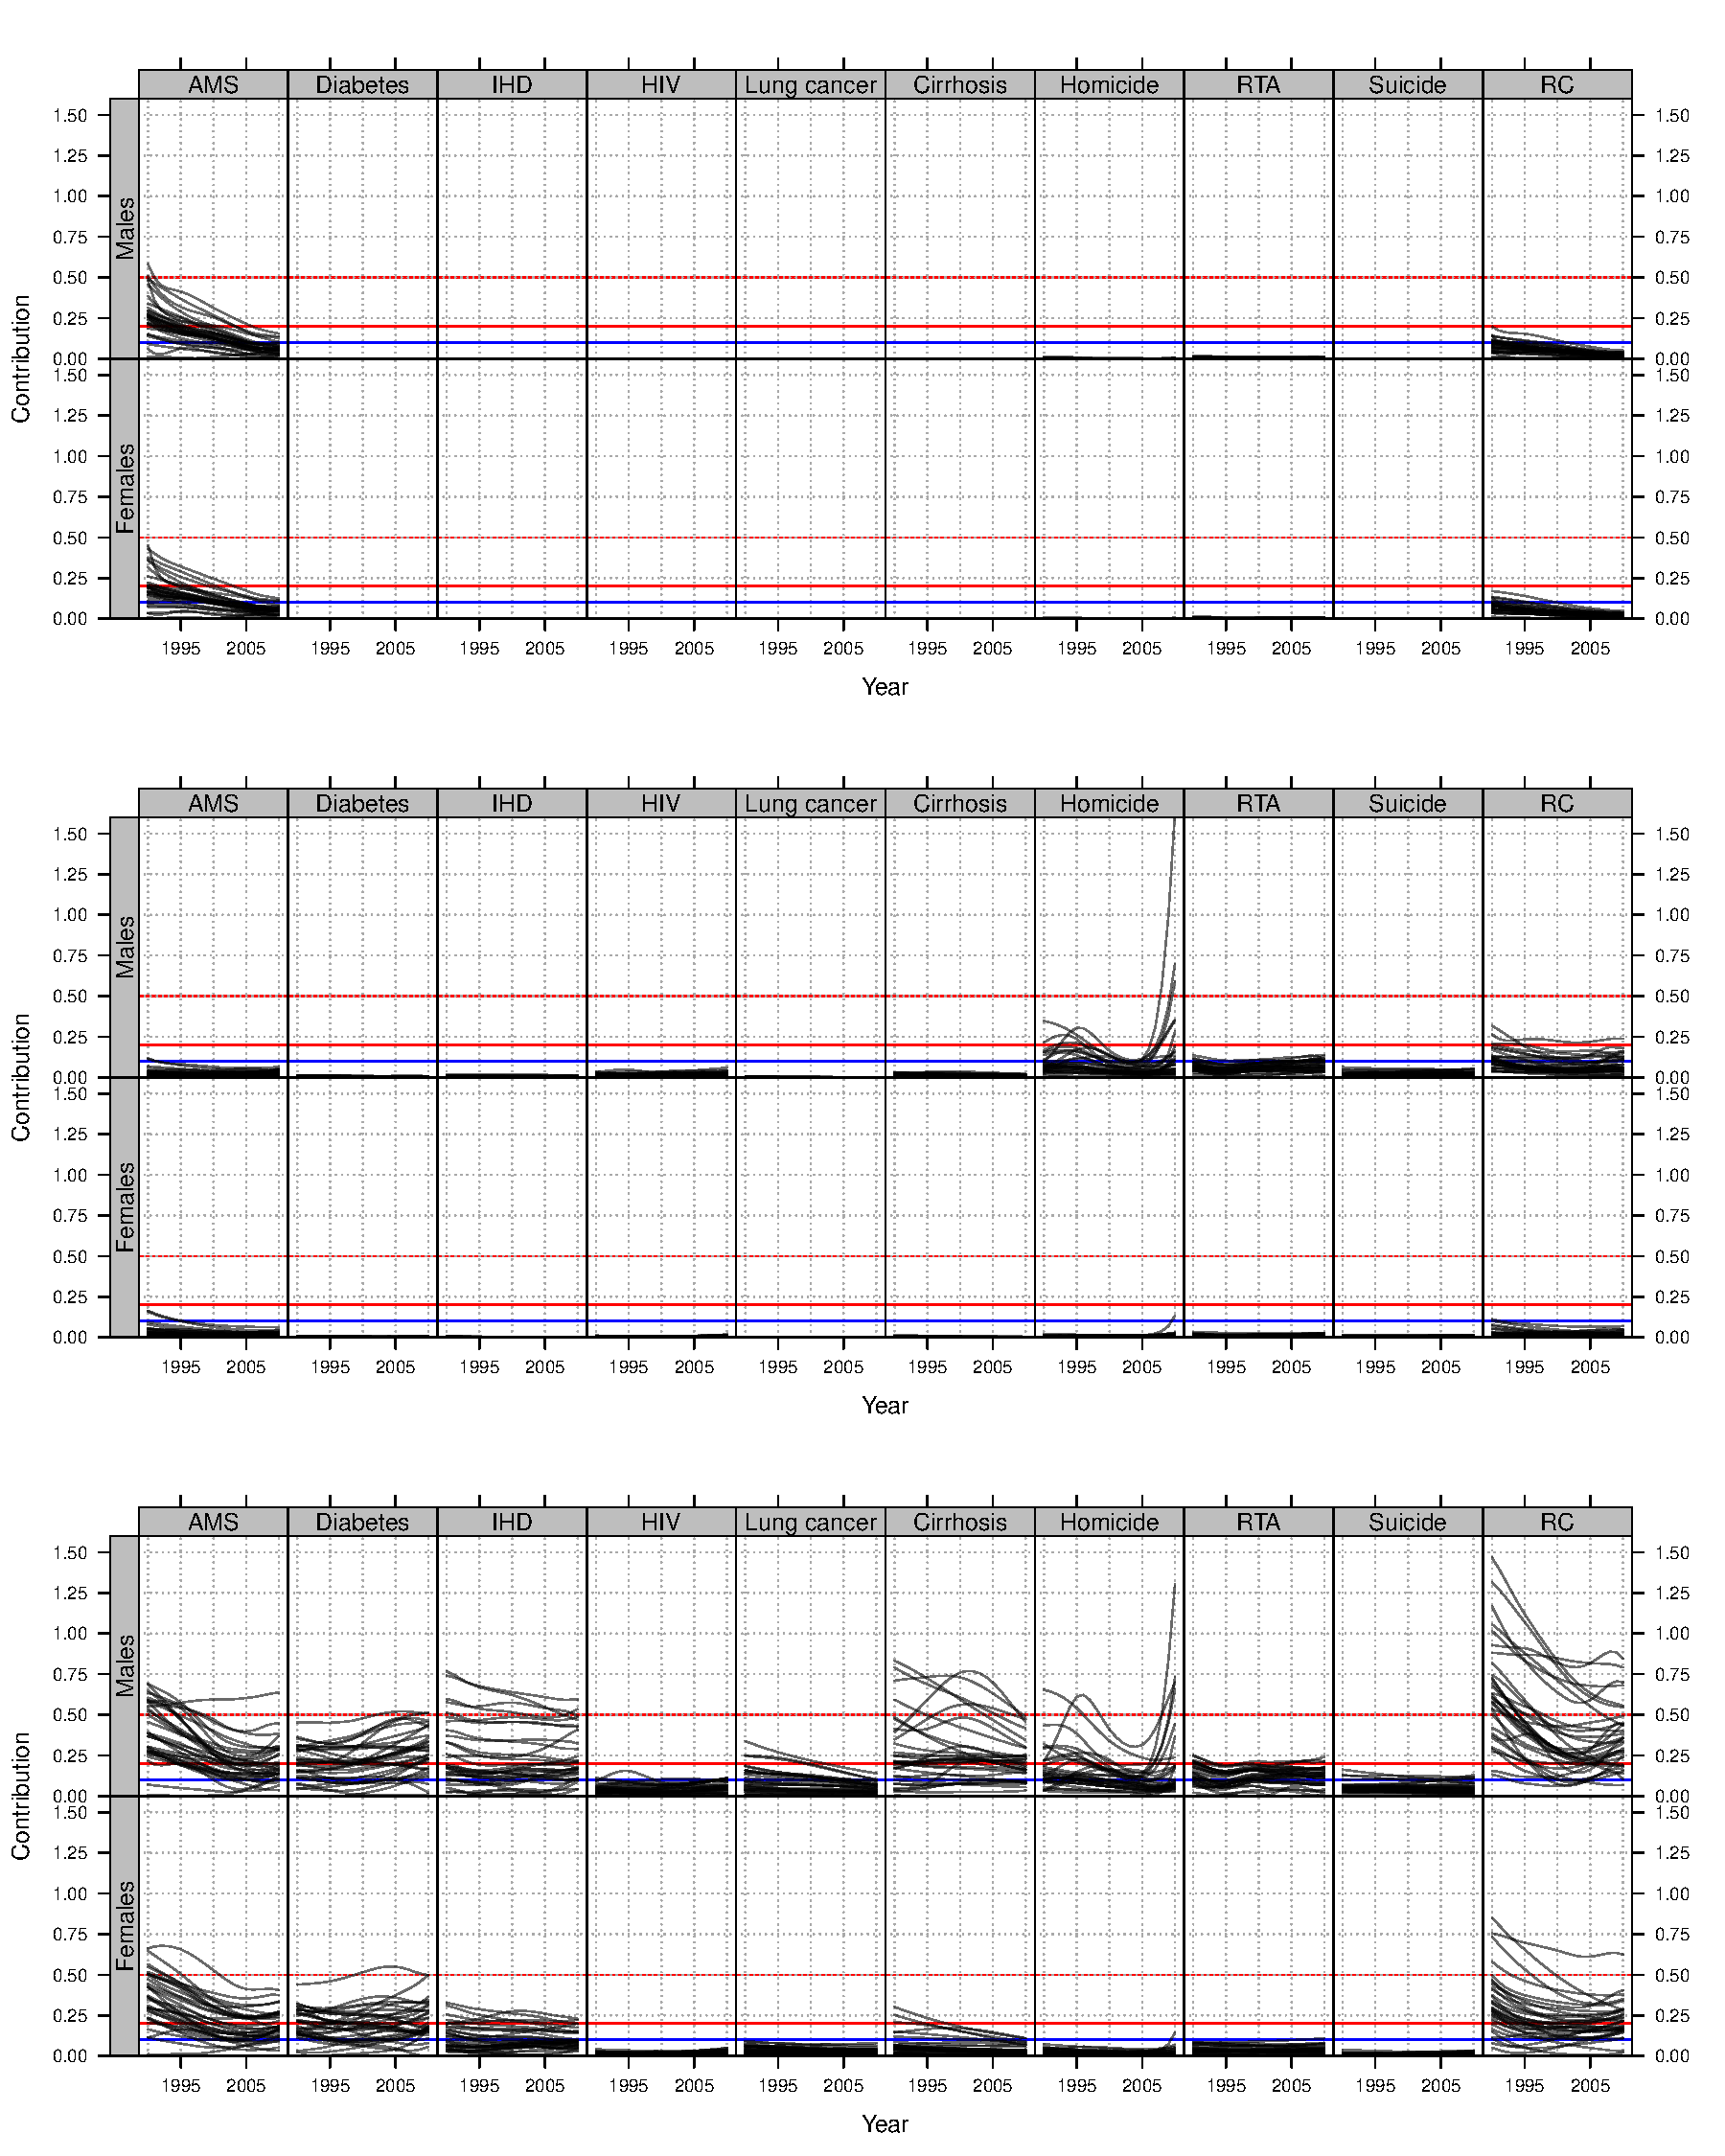
\includegraphics[scale=.4]{Figures/TLE_Decomp.pdf}
%Source: own calculations based on INEGI and SOMEDE
%\end{figure}


%This will show a few small multiples figures, tbd 

%\section*{Discussion}
%Talk about the role of homicide and other major causes. How many years of life
%were lost? (not just expectancy). maybe..

\section*{Discussion}
\subsection*{Child and young-adult mortality}

This analysis demonstrates the potential contribution of achieving the low mortality benchmark to improvements in survival. However, it is concerning that the low mortality benchmarks have not been steadily increasing over the period studied. Trends were flat for children, they are experiencing almost full survival before age 15. More worrisome is the common shift after 2005 in adults aged 15-39 and decreasing survival among older adults aged 35-74.

Despite the flattening pattern of the low mortality benchmark in children, our results show that all states in Mexico have improved survival towards this benchmark and to the maximum survival. Causes amenable to medical service are at the heart of such improvements, consistent with decreases in infectious and respiratory diseases associated with public health interventions targeted to children in Mexico previously documented \cite{sepulveda2006}. For example, Puebla and Tlaxcala improved survival over half a year since the 1990's. By 2010 survival was improved so that all states' temporary life expectancy ranged between 14.6 and 14.8 years. We further estimated survival inequalities between states by age group calculating Gini coefficients for every year (Figure \ref{fig:Gini}).  Indeed, survival equality before age 15 is almost achieved paralleling improvements in mortality rates during the period. In addition, our results are also consistent with advances in coverage for skilled attendance at delivery, which by 2012 remained above 90\% and more than 78\% of children under age one visited the doctor to monitor their development and growth  \cite{urquieta2015evolution}. Moreover, vaccination coverage has been achieved for the entire young population, the success of such public health interventions are in line with our results, underscoring the improvements in survival in the population younger than 15 years associated to the progress detected in health insurance coverage due to vaccination programs and the implementation of the Seguro Popular \cite{urquieta2015evolution}. Although average years lived below 15 has improved, there still exist areas of opportunity to achieve full-survival under age 15 in causes amenable to medical service, mainly in states in the Central and Southern regions of the country. 


\subsection*{Older-adult mortality}

Adults aged 15-39 show a converging pattern towards the low mortality benchmark in all states just until 2005. A sudden increase in homicide rates widened the gap with the low mortality benchmark by almost four times on average in 2010 relative to the level observed in 2005. Previous research documented losses in the overall life expectancy up to three years in the state of Chihuahua (the bordering state with Texas, USA) and almost two years in Sinaloa, Durango (North) and Guerrero (South) between 2005 and 2010 due to homicides \cite{Aburto2015}. Our findings show that the trend towards the low mortality benchmark was reversed after 2005 due to the increase in homicide mortality, with a peak in 2011. Although homicide rates decreased after 2011, they still are the main cause of death contributing to the gap between the observed survival and the low mortality benchmark in particular states, such as Sinaloa, Durango in the North, Nayarit and Michoac\'an in the cetral region, and Guerrero in the South. These findings underscore the need for effective interventions to reduce homicide mortality, as it still contributes the most to survival shortcomings among the young-adult population and mortality inequality among states. Even ten years after the national security strategy that aimed at reducing drug cartels' operations started and homicides begun to spread all over the country \cite{espinal2015analysis}, the effect of homicide on average survival is appalling. Between-state inequality in female survival was much smaller over the same period (figure \ref{fig:Gini}), though females showed the same overall trend of convergence, followed by divergence after 2005. 


%rember capital letters to norht, south, etc..
In Mexico, since the beginning of the 1990's, adult survival in ages 40-74 deteriorate for males and stagnate for females. Our results help explain on this pattern showing that the low mortality benchmark decreased as a result of state-specific mortality trends and the interaction between specific causes of death. In particular, there are offsetting effects between improvements in causes amenable to medical service, such as infectious and respiratory diseases, and deterioration in diabetes, isquemic heart diseases (IHD), and behavior-related mortality through cirrhosis and homicides. 

Out of 35 potential years, adult females in Mexico are living less than 33 and males less than 31 since the 1990's. The increase in  diabetes, IHD and cirrhosis mortality is at the heart of survival's deterioration, with clear regional variations. Although improvements in causes amenable to medical service were witnessed, almost every state still has potential to improve in this ages, in particular the Northern states of Sonora, Chihuahua and Baja California. Diabetes mortality increased over the period and contributed to increases in the gap to achieve the low mortality benchmark. Diabetes-related mortality increased 23\% from 1998 to 2002, and the prevalence of diabetes was estimated at 14.4\% in the adult population in 2006. These figures underscore the emerging epidemic of diabetes \cite{glassman2010confronting}. To put this in perspective, Coahuila, the state of Mexico, Guanajuato, the Federal District, Tabasco and Puebla could increase survival by almost one year if diabetes mortality were to achieve the low mortality benchmark. Similarly, mortality related to IHD contributes to lowering life expectancy in adults. There is a clear regional pattern in the country. Almost all the states in the Northern region could potentially benefit with one additional year in life expectancy if the low mortality benchmark were reached, where as the Central and Southern regions present a lower impact of IHD. Cirrhosis-related mortality shows a higher impact in the Southern and Central states of the country, particularly in Quer\'etaro, M\'exico state, Hidalgo (central area) and Puebla and Oaxaca in the South. Both diabetes and IHD mortality are closely related to obesity prevalence, previous research anticipated that the increasing levels of obesity in Mexico could compromise gains in life expectancy \cite{monteverde2010obesity}. These regional differences on cause-specific mortality led to increases in health inequalities in adults aged 30-74 after 2006 for males and stagnation among females (figure \ref{fig:Gini}). 


There is still potential for improvements to reduce state-mortality differences and improve the survival among the adult population in Mexico. Several screening and prevention strategies (e.g. PREVENIMSS) for early diabetes and hypertension have been implemented in the country. However, as previous research has found, they are far from achieving the ultimate goal and including the entire population \cite{castro2010potential}. In addition, \cite{behrman2013health} show that the conditional cash transfer program PROSPERA improves health significantly for adult women older than 50. The authors also noted that the effect on men's health is much lower. They argue that this could be the result of the lack of inclusion of men in the program and the main role of women in the program's requirements. Women are recipients of the monetary transfers and they are more likely to attend clinic visits and follow health measures given by doctors in these clinics than men.\\

\begin{center}
[Figure \ref{fig:Gini} about here]
\end{center}

\section*{Conclusion}
Improving health is a priority for governments of many developing countries. In part to reduce child mortality, improve maternal health and lessen the impact of other infectious diseases, such as HIV/AIDS, to achieve the Millennium Development Goals established for 2015 \cite{united2009millennium}.  Mexico has succeeded in reducing mortality and inequalities in children and the young population. Nevertheless, our results show that older adults are becoming a vulnerable group, and more efforts are required to reduce the burden of conditions amenable to health services and policy-related conditions. In particular, this group lacks comprehensive interventions to reduce the burden of violence through homicides, chronic-degenerative
causes of death, such as diabetes and IHD, and behavior-related conditions such as cirrhosis.  

There is no simple way to lessen the impact of such conditions, but it is clear that new approaches are needed to improve survival in the adulthood and to minimize health disparities between states. Preventing diabetes and IHD implies fundamental political challenges. Therefore,  public health initiatives should focus in health care for chronic conditions as recently suggested by \cite{knaul2015achieving}, but they should also influence the population towards improving health behavior. Our results reinforce the need of such, among others public health interventions, with an special focus on older adults in the Mexico. 

%\nocite{oreg,schn,pond,smith,marg,hunn,advi,koha,mouse}

%%%%%%%%%%%%%%%%%%%%%%%%%%%%%%%%%%%%%%%%%%%%%%
%%                                          %%
%% Backmatter begins here                   %%
%%                                          %%
%%%%%%%%%%%%%%%%%%%%%%%%%%%%%%%%%%%%%%%%%%%%%%

\begin{backmatter}

\section*{Competing interests}
  The authors declare that they have no competing interests.

\section*{Author's contributions}
 JMA and TR conceptualized the study, performed the analyses and wrote the manuscript.

\section*{Acknowledgements}
  Text for this section \ldots
%%%%%%%%%%%%%%%%%%%%%%%%%%%%%%%%%%%%%%%%%%%%%%%%%%%%%%%%%%%%%
%%                  The Bibliography                       %%
%%                                                         %%
%%  Bmc_mathpys.bst  will be used to                       %%
%%  create a .BBL file for submission.                     %%
%%  After submission of the .TEX file,                     %%
%%  you will be prompted to submit your .BBL file.         %%
%%                                                         %%
%%                                                         %%
%%  Note that the displayed Bibliography will not          %%
%%  necessarily be rendered by Latex exactly as specified  %%
%%  in the online Instructions for Authors.                %%
%%                                                         %%
%%%%%%%%%%%%%%%%%%%%%%%%%%%%%%%%%%%%%%%%%%%%%%%%%%%%%%%%%%%%%

% if your bibliography is in bibtex format, use those commands:
\bibliographystyle{bmc-mathphys} % Style BST file (bmc-mathphys, vancouver, spbasic).
\bibliography{AburtoRiffe_Bib}      % Bibliography file (usually '*.bib' )
% for author-year bibliography (bmc-mathphys or spbasic)
% a) write to bib file (bmc-mathphys only)
% @settings{label, options="nameyear"}
% b) uncomment next line
%\nocite{label}

% or include bibliography directly:
% \begin{thebibliography}
% \bibitem{b1}
% \end{thebibliography}

%%%%%%%%%%%%%%%%%%%%%%%%%%%%%%%%%%%
%%                               %%
%% Figures                       %%
%%                               %%
%% NB: this is for captions and  %%
%% Titles. All graphics must be  %%
%% submitted separately and NOT  %%
%% included in the Tex document  %%
%%                               %%
%%%%%%%%%%%%%%%%%%%%%%%%%%%%%%%%%%%

%%
%% Do not use \listoffigures as most will included as separate files

\section*{Figures}

\begin{figure}[h!]
\centering
\caption{Temporary life expectancy for states (black line), record life
expectancy (red) and low mortality benchmark by sex, 1990-2010.}
\label{Fig1:temp}

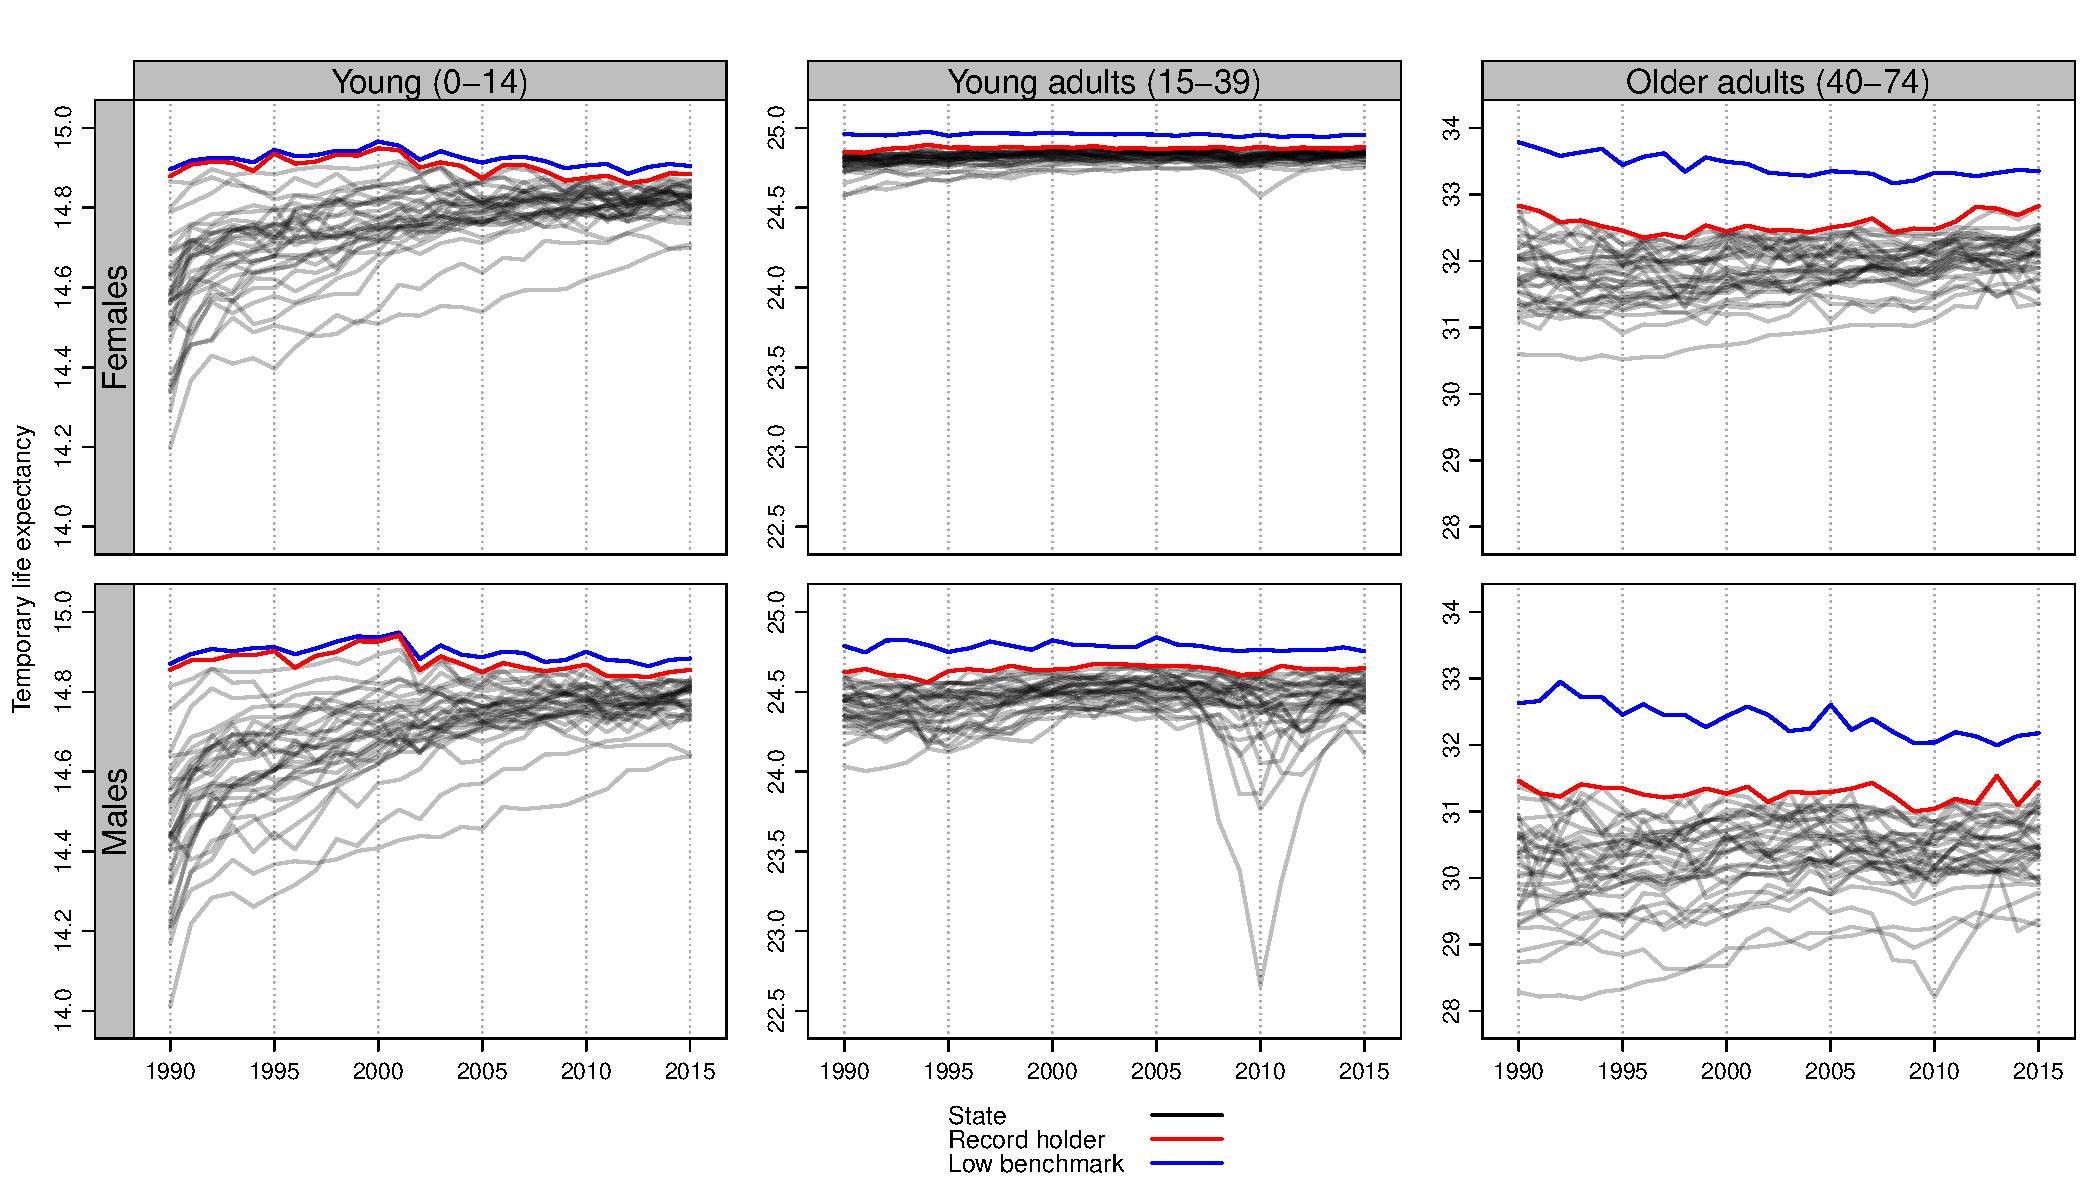
\includegraphics[scale=.35]{Figure1.pdf}

Note: Y-axis are not in the same scale in order to capture major trends over the period. Source: calculations based on INEGI and SOMEDE files. 
\end{figure}



\begin{figure}[h!]
\centering
\caption{Survival inequality (coefficient of variation) by age group and sex, 1990-2010.}
\label{fig:Gini}
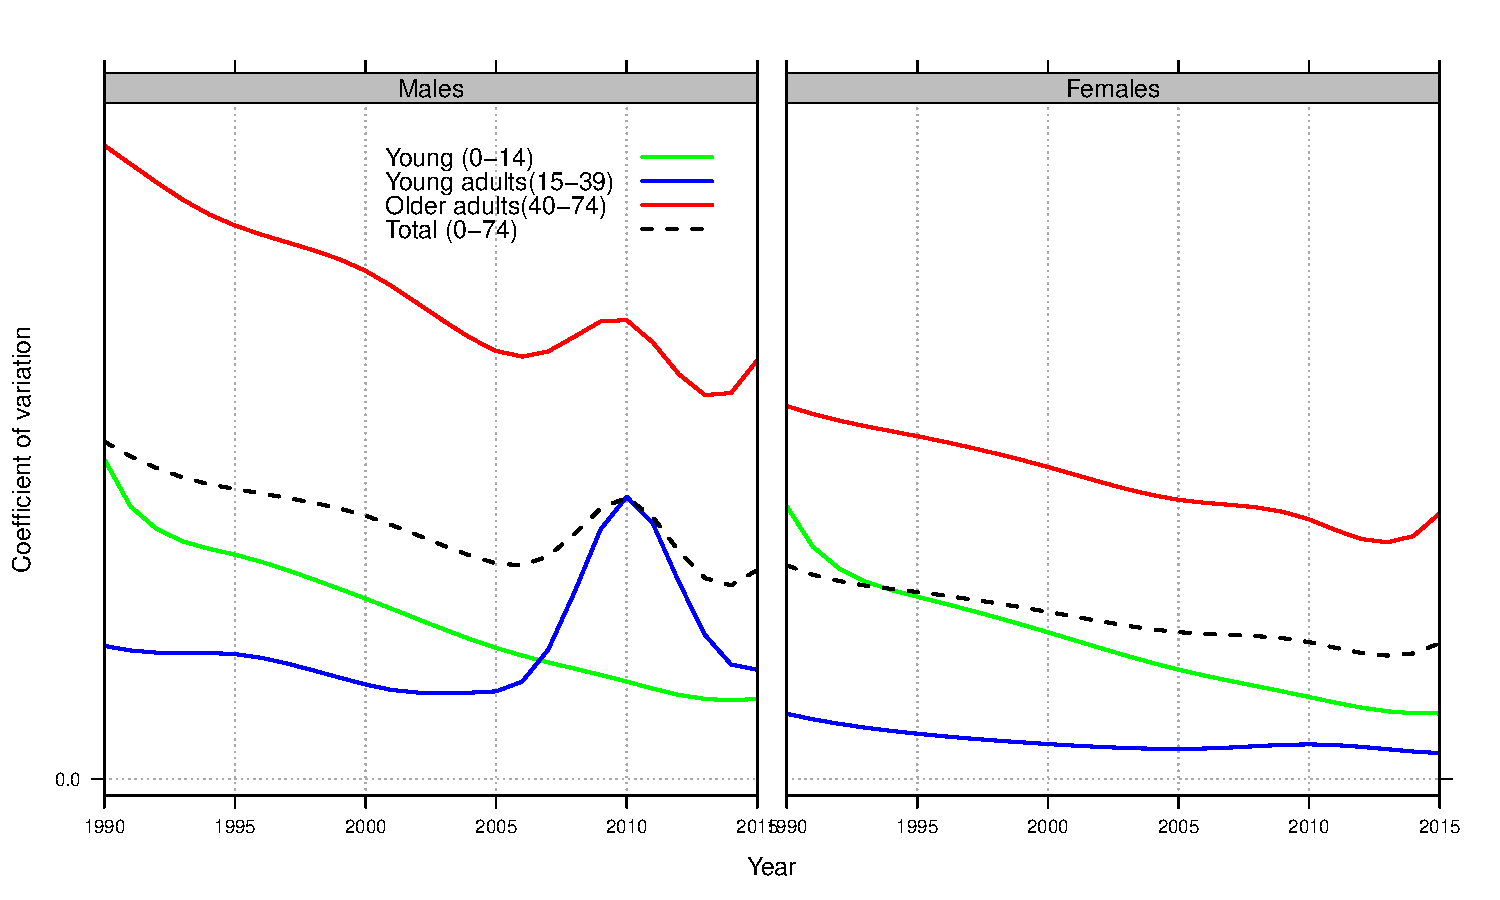
\includegraphics[scale=.4]{CVfig.pdf}

 Source: calculations based on INEGI and SOMEDE files.
\end{figure}



\begin{figure}[h!]
\centering
\caption{Cause-specific contributions to state differences from low mortality benchmark for older male adults, 1990-2010.}
\label{fig:e40_74_males}

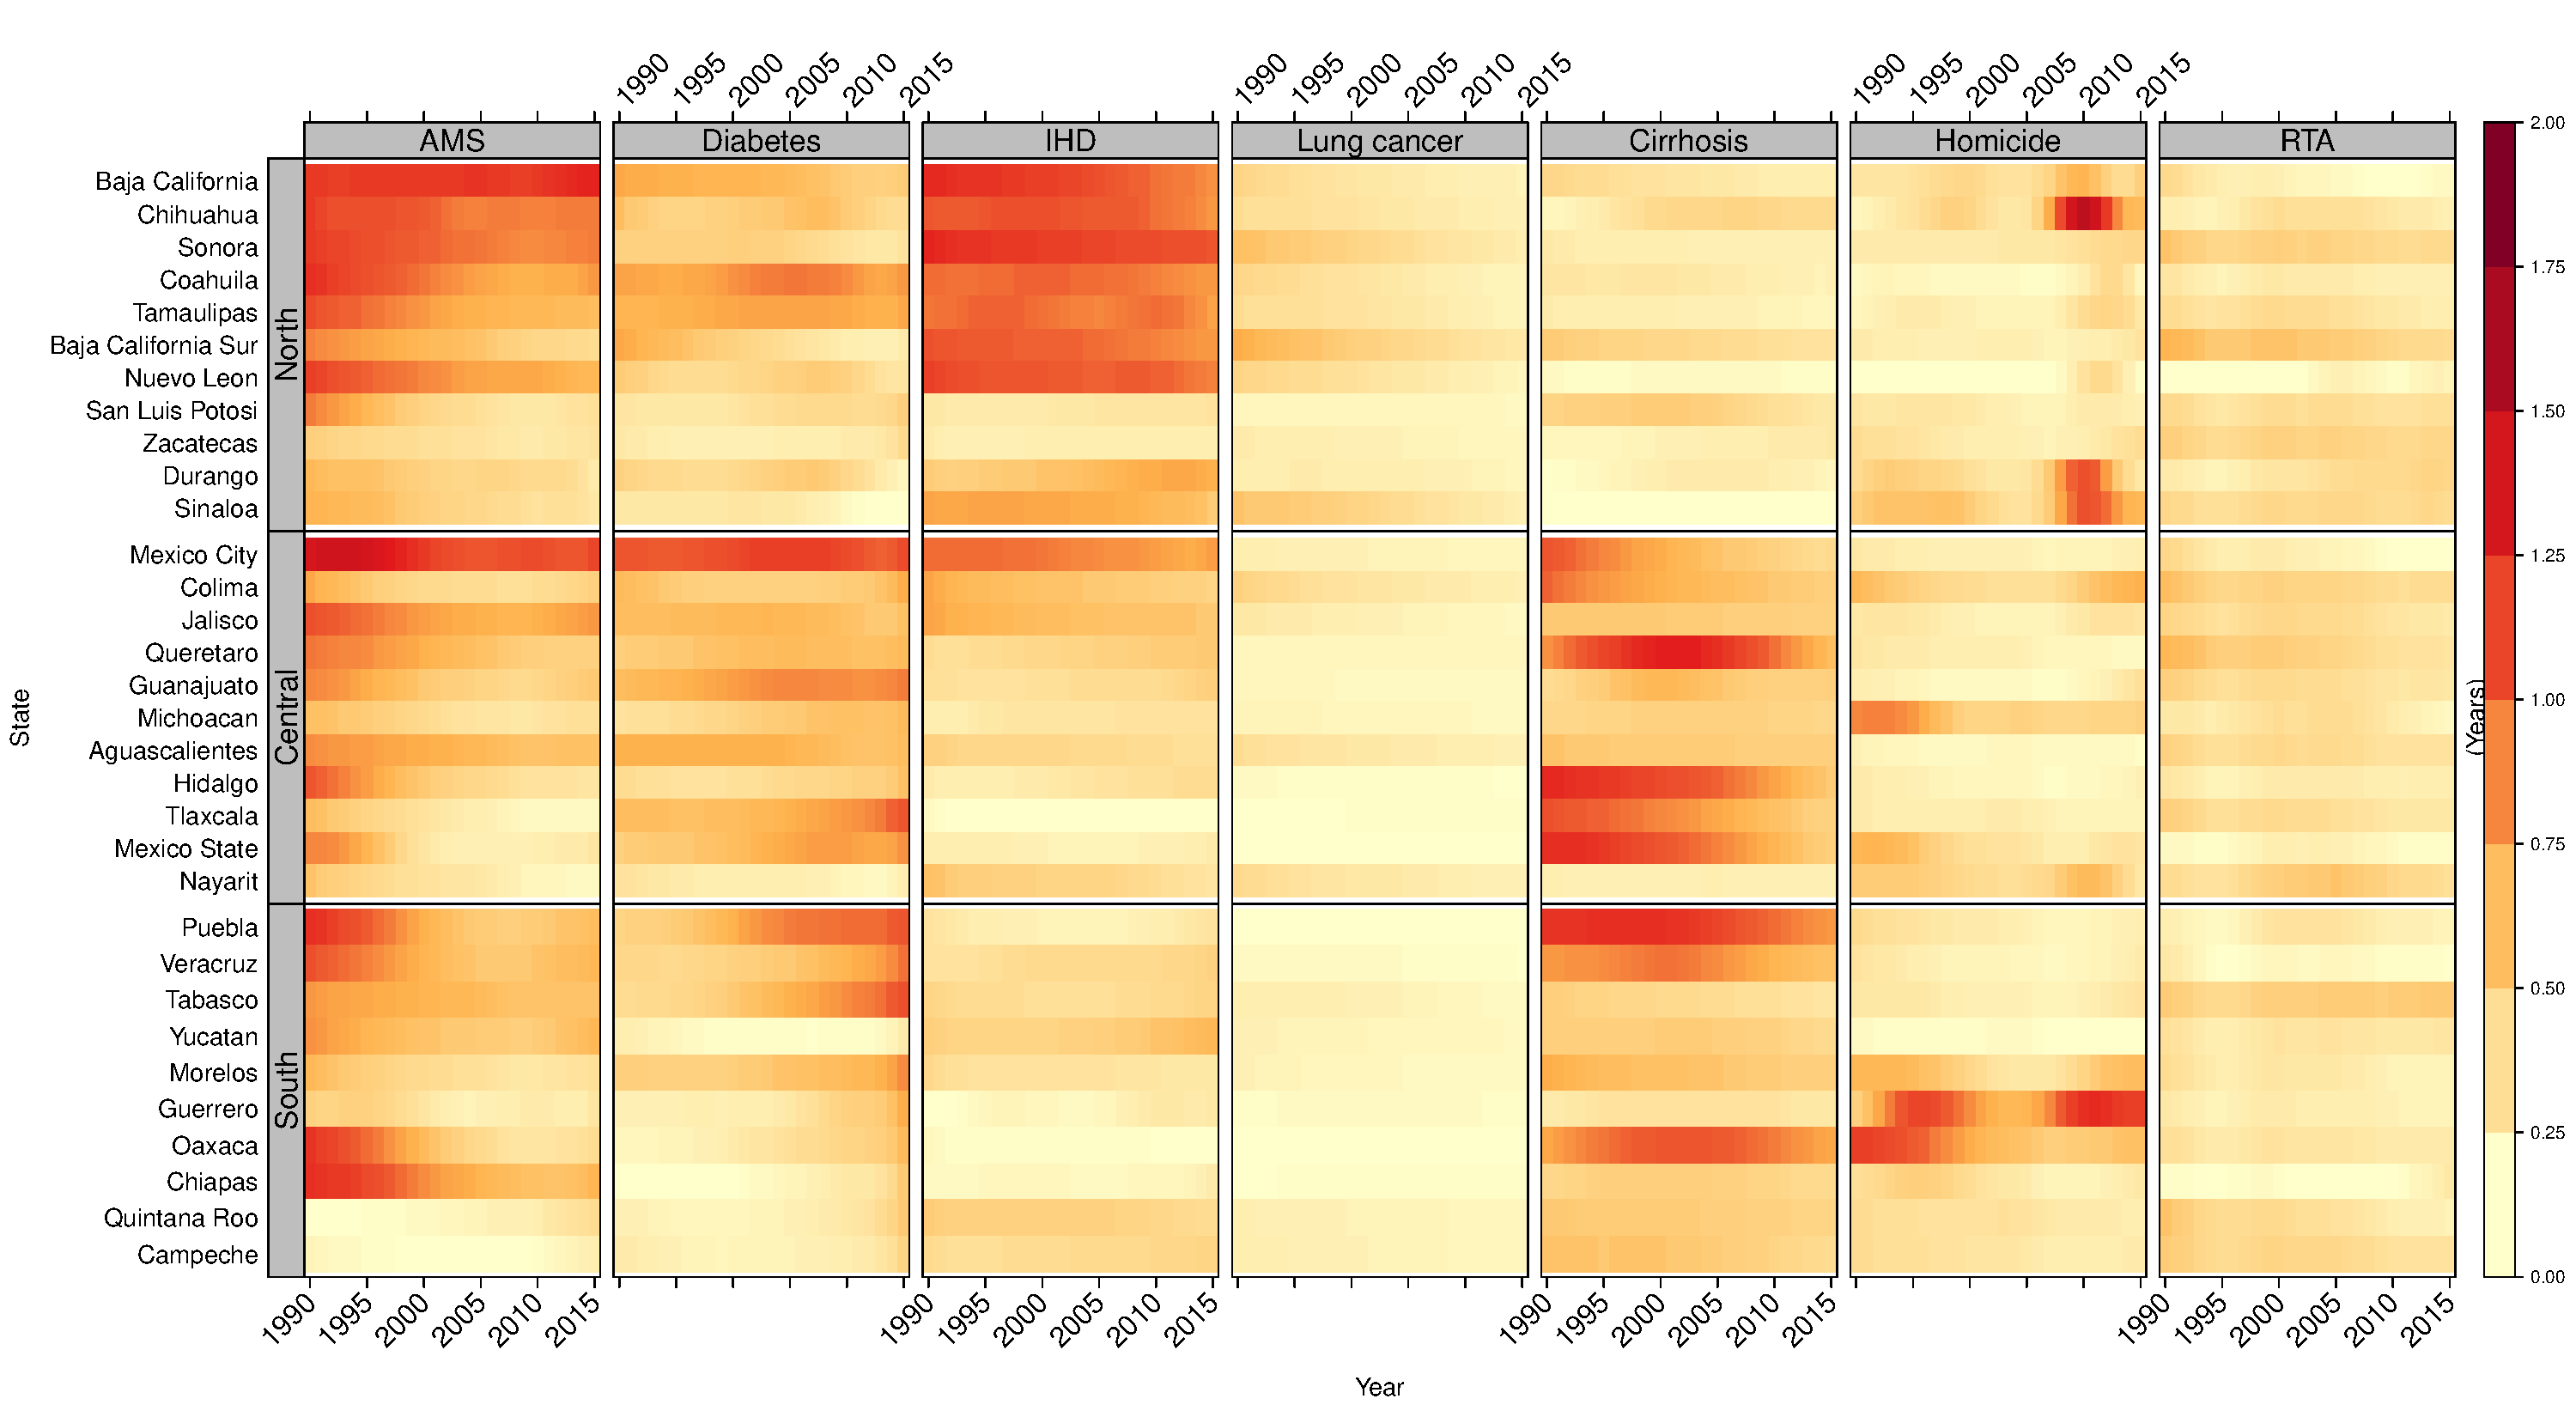
\includegraphics[scale=.23]{AdultMaleheatmap.pdf}
Note: AMS, is the acronym for amenable to medical service, IHD for isquemic heart diseases and RTA stands for road traffic accidents. Source: own calculations based on INEGI and SOMEDE files. 
\end{figure}

%%%%%%%%%%%%%%%%%%%%%%%%%%%%%%%%%%%
%%                               %%
%% Tables                        %%
%%                               %%
%%%%%%%%%%%%%%%%%%%%%%%%%%%%%%%%%%%

%% Use of \listoftables is discouraged.
%%
\section*{Tables}
% latex table generated in R 3.3.1 by xtable 1.8-2 package
% Wed Jan 18 14:53:15 2017
\begin{table}[ht]
\centering
\caption{Avoidable Mortality classification, 
             with crude percentages below age 75, years 1990-2015. Source: INEGI files.} 
\label{tab:causes}
\begin{tabular}{llllll}
  \hline
& Category &\% & Males &  \% & Females \\ 
 &&& (1,000's) & & (1,000's)\\ 
  \hline
1&  Causes amenable to medical service & 30.9 \% & 127.5 & 28.2 \% & 114.4 \\ 
2&  Diabetes & 4.5 \% & 18.7 & 4.9 \% & 19.9 \\ 
3&  Ischemic heart diseases & 4 \% & 16.4 & 4.2 \% & 17 \\ 
4&  HIV/AIDS & 0.4 \% & 1.5 & 0.5 \% & 2.1 \\ 
5&  Lung cancer & 0.9 \% & 3.7 & 0.9 \% & 3.8 \\ 
6&  Cirrhosis & 2.3 \% & 9.5 & 2.5 \% & 10 \\ 
7&  Homicide & 2.7 \% & 11.2 & 3 \% & 12.4 \\ 
8&  Road traffic accidents & 2.8 \% & 11.4 & 2.9 \% & 11.8 \\ 
9&  Suicide & 0.4 \% & 1.7 & 0.5 \% & 1.9 \\ 
10&  Other causes & 24.8 \% & 102.4 & 25 \% & 101.2 \\ 
   \hline
\end{tabular}
\end{table}

%%%%%%%%%%%%%%%%%%%%%%%%%%%%%%%%%%%
%%                               %%
%% Additional Files              %%
%%                               %%
%%%%%%%%%%%%%%%%%%%%%%%%%%%%%%%%%%%

\section*{Additional Files}
  \subsection*{Additional file 1 --- Supplemental material}
   This might refer to a multi-page table or a figure.

  \subsection*{Additional file 2 --- Results}
 Rdata file with all results.


\end{backmatter}
\end{document}
